\documentclass[convert]{standalone}

\usepackage{tikz}
\usetikzlibrary{backgrounds}
\usepgflibrary{shadings} 

\begin{document}

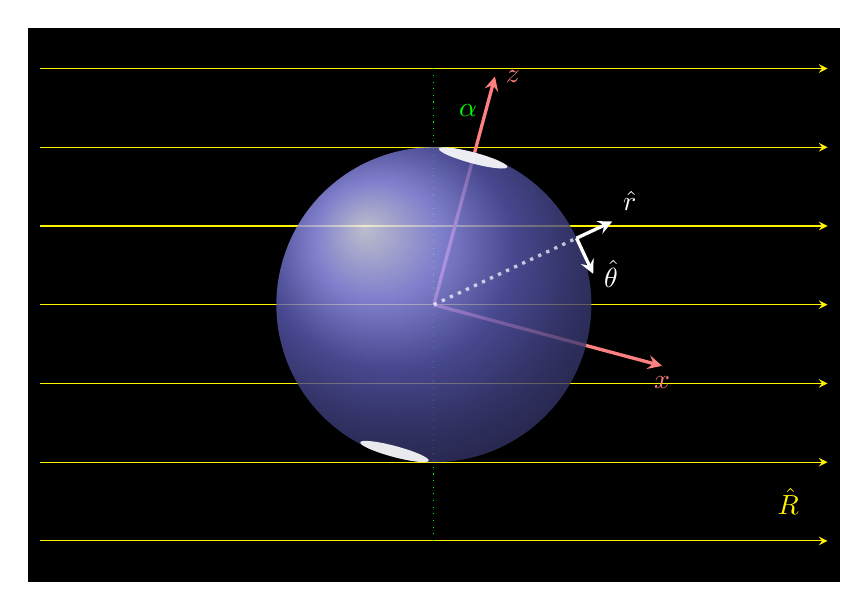
\begin{tikzpicture}[background rectangle/.style={fill=black}, show background rectangle,>=stealth]
  \node at (0,3.25) {};
  \node at (0,-3.25) {};

  \foreach \i in {-3,-2,...,3}{
    \draw[yellow,->] (-5,\i) -- (5,\i);
  }
  \node at (4.5,-2.5) [yellow]{$\hat{R}$};

  \draw[green, dotted] (0,-3) -- (0,3);

  \begin{scope}[red!50!white, very thick,rotate=-15]
    \draw[->] (0,0) -- +(3,0) node[below]{$x$};
    \draw[->] (0,0) -- +(0,3) node[right]{$z$};
    \shade[ball color=blue!50!white,opacity=0.8] (0,0) circle (2);
    \fill[white,opacity=0.9] (0,1.93) ellipse (0.45 and 0.07);
    \fill[white,opacity=0.9] (0,-1.93) ellipse (0.45 and 0.07);
    \draw[->,white!90] (40:2) -- +(40:0.5) node[above right]{$\hat{r}$};
    \draw[->,white!90] (40:2) -- +(-50:0.5) node[right]{$\hat{\theta}$};
    \draw[white!90,dotted,opacity=0.7] (0,0) -- (40:2);
  \end{scope}
  \node at (80:2.5) [green]{$\alpha$};
\end{tikzpicture}

\end{document}

